\hypertarget{earlyexiting}{%
	\chapter{Edge Offloading with Early Exiting}\label{ch:edgeoffloading}}
\thispagestyle{fancy}

In this chapter we implement an inference scheme utilizing early exiting \gls{dnn}s. Our scheme is flexible in the sense it can be used in different edge-centric architectures and it is adaptive to enable service at more stringent latency requirements than currently proposed in literature using a best effort approach. In section \ref{sec:edge-aee} we present our offloading scheme In section \ref{sec:edge-system-model} we define the system model used to evaluate our result. We describe our implementation in section \ref{sec:edge-implementation} In section \ref{sec:edge-exp-setup} we describe our experimental setup. In section \ref{sec:edge-results} we present our results and in section \ref{sec:edge-summary} we discuss our results.

\section{\acrfull{aee} for Time-Critical Applications} \label{sec:edge-aee}

We propose \acrfull{aee} an optimistic inference scheme based on early exit \gls{dnn}. It is optimistic, as it maximizes the reliability using a best effort apporach. The scheme does not terminate at early exits, but when a deadline has passed. Thus, the inference is run until time is out. The scheme  allow to use increasingly confident predictions from the continuous inference process. Our scheme is flexible at it can function for on-device, edge offloading or collaborative inference architectures. 

\begin{figure}
	\captionsetup[subfigure]{justification=centering}
	\centering
	\subfloat[Continuois predictions\label{fig:offloading-scheme-successful}]{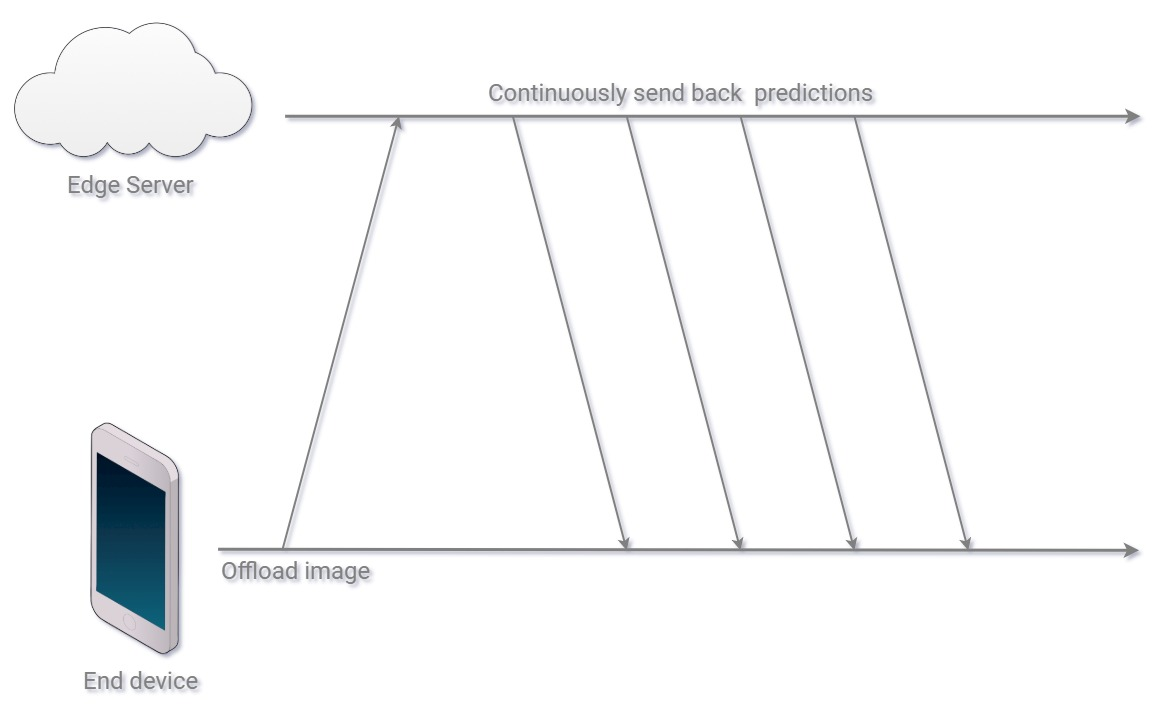
\includegraphics[width=.7\linewidth]{figures/models/timeline_all}}
\end{figure}
\begin{figure}
		\captionsetup[subfigure]{justification=centering}
	\centering
	\subfloat[Timeout of Continuois predictions\label{fig:offloading-scheme-timeout}]{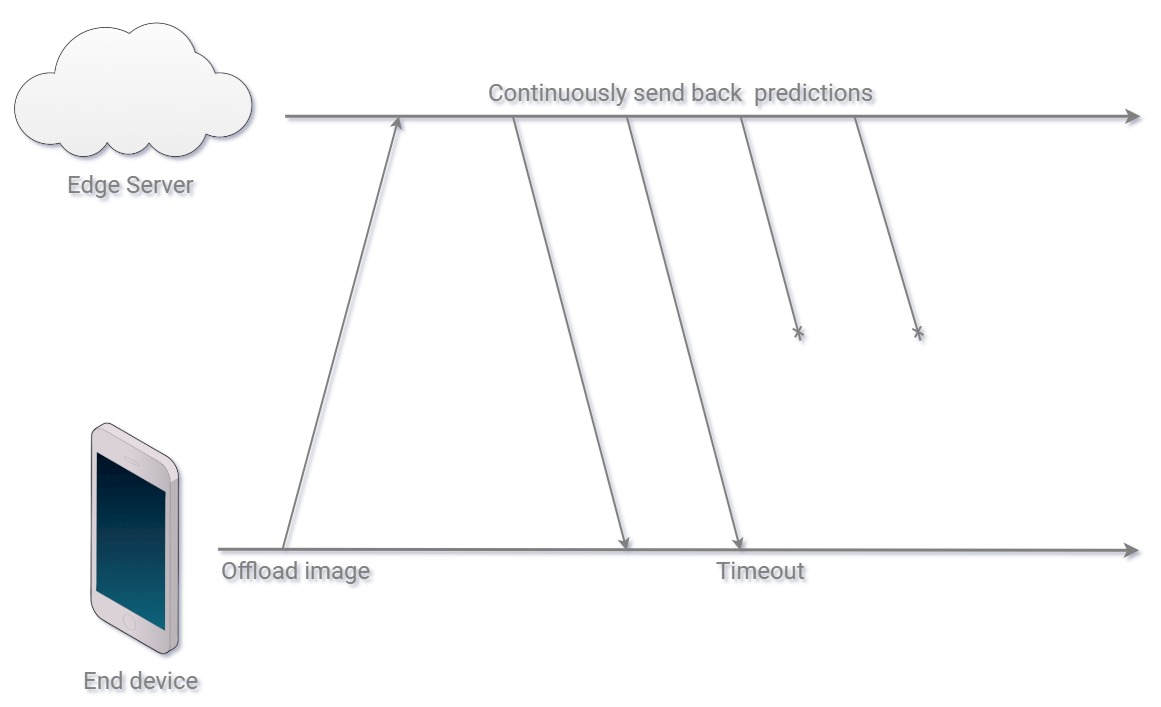
\includegraphics[width=.7\linewidth]{figures/models/timeline_timeout}}
	\caption[Offloading scheme]{offloading scheme}
	\label{fig:offloading-scheme}
\end{figure} 

We present the scheme in the context of edge offloading llustrated in figure \ref{fig:offloading-scheme}. The data is immediately offloaded upon acquisition from the end device to edge server, to not waste idle time on edge server. The edge server runs the inference process, and whenever a prediction is obtained from the early exit \gls{dnn} classifers, it is sent back to the end device. Successively receiving prediction allow the user to select the most recent prediction from the deepest exit. Or alternatively, use information from all received predictions to select the most confident or use a combination function to select the best one. Figure \ref{fig:offloading-scheme-successful} illustrates the continuous reply of predictions. Figure \ref{fig:offloading-scheme-timeout} illustrates a case, where a timeout occurs and only two predictions are available 

In the next section we define the system model.

\section{System Model} \label{sec:edge-system-model}

In this section we define the system model for \gls{aee}. Note the metrics defined in chapter \ref{ch:earlyexit} is reused. To remind the reader:  $ C $ denotes the number of the image classes, $ N $ denotes the number of the exit points in a DNN, $ I $ denotes the number of images. 

We still do not differentiate between early exit and conventional model,  as we use $ T_{i,n}^{cmp} $ to denote computation time irregardless of conventional inference model with a single exit, or early exit models with multiple. We do extend our view on latency, as we introduce two execution schemes.
	
	\begin{enumdescript}
		\item[Latency]  We have two options \textbf{A)} local processing and \textbf{B)} edge offloading. Hence we denote the computation time for local processing $ T_{i,n}^{loc,cmp} $ and $ T_{i,n}^{edge,cmp} $ to denote computation time at the edge. 
	
		We define the time for local and remote execution

		\begin{enumdescript}
			\item[Local Execution] If the classification exits from exit point $ n $, the processing delay of image $ i $ at local is presented as
			\begin{align}
			T_{i,n}^{loc}= T_{i,n}^{cmp,loc}
			\end{align}
			\item[Remote Execution] If the classification exits from exit point $ n $, the processing delay of image $ i $ at edge is presented as
			\begin{align}
			T_{i,n}^{edge}=T_{i}^{com}+ T_{i,n}^{cmp,edge}
			\end{align}
			where $ T^{com}_i $ denotes the communication time, for both uplink time to transmit image $ i $ from local to edge, and downlink time of prediction reply from edge to local.
			
			Offloading for remote execution is only sensible whenever we save time compared to local execution, i.e.
			\begin{align*}
					T_{i,n}^{loc} > T_{i,n}^{edge}
			\end{align*}
			\todo{should I denote this a sub T^{cmp}_n? as there are downlink communication every time a prediction is acquired. Or split it in downlink and uplink?}
			Due to the difference in computing resources, we expect the computation time at edge to be significantly lower than local computation time, i.e. $ T_{i,n}^{loc,cmp} > T_{i,n}^{edge,cmp} $. Thus, the communication time $ T^{com}_i $ becomes an important factor for offloading decision.

		\end{enumdescript}
	
		\item[Accuracy] The scheme allow for the opportunities to receive multiple predictions within the time frame. We may be able to improve the accuracy and reduce undesired overthinking, using the output results of the first $ n $ exit points to combine the information.
		
		\begin{align}
		\bar{A}^f &= 1 - \frac{1}{I} \sum_{i=1}^{I}\mathbb{I}\left(\left|f\left(\bm{\hat{y}}_{i,1} \dots, \bm{\hat{y}}_{i,n}\right)-c_i\right|\right)
		\end{align}
		
		remember the ground truth class label of image $ i $ is $ c_i \in \left\{1, 2, C \right\} $ and $ \mathbb{I(\cdot)}  $ is a indicating function defined by in eq. \ref{eq:indicator}.
		\begin{align*}
		\mathbb{I}(a)= \begin{cases}
		0, & \mathrm{if\:} a \leq 0, \\
		1, & \mathrm{otherwise}
		\end{cases}
		\end{align*}
		
		There are several ways to define combination function $ f\left(\bm{\hat{y}}_{i,1}, \dots, \bm{\hat{y}}_{i,n}\right) $
		\begin{enumdescript}
			
			
			\item[Latest] We define the method \emph{lastest}, where we constrain ourselves to only use the most recent prediction $n$.
			\begin{align}
			f\left(\bm{\hat{y}}_{i,1}, \dots, \bm{\hat{y}}_{i,n} \right) = \hat{c}_{i,n}^{*}
			\end{align}
			
			\item[max confidence] This method uses the most confident prediction among all received exit predictions. It is used in \cite{kaya_shallow-deep_nodate}, which reports improvement on the \gls{cifar10}, \gls{cifar100} and \gls{tinyimagenet}. The measure is based on the assumption, that an exit obtaining a higher score is more confident, hence improving the accuracy.
			\begin{align}
			\begin{split}
			f\left(\bm{\hat{y}}_{i,1}, \cdots, \bm{\hat{y}}_{i,n} \right) =  \arg \underset{c}{\max} \{\hat{y}^*_{i,1}, ..., \hat{y}^*_{i,C} \},
			\\ \text{where\:} \hat{y}^*_{i,c} = \max \{\hat{y}_{i,1,c}, ..., \hat{y}_{i,n,c}\}
			\end{split}	
			\end{align}
			\item[sum confidence] this method sums the respective class scores for all exit predictions and chooses the highest scoring class. 
			\begin{align}
			\begin{split}
			f\left(\bm{\hat{y}}_{i,1}, \dots, \bm{\hat{y}}_{i,n} \right) = \arg \underset{c}{\max} \{s_{i,1}, \dots, s_{i,C}\}, \\ \text{where\:} s_{i,n} = \sum_{j=1}^{n}\hat{y}_{i,n,c} \forall \ 1\le c \le C
			\end{split}
			\end{align}
			
			%				\item[weighted sum confidence] this method perform a weighted sums of the respective class scores for all exit predictions and chooses the highest scoring class. 
			%
			%				\begin{align}
			%				\begin{split}
			%					f\left(\bm{\hat{y}}_{i,1}, \dots, \bm{\hat{y}}_{i,n} \right) = \arg \underset{n}{\max} \{s_{i,1}, \dots, s_{i,C}\},\\ \text{where\:} s_{i,n} = \sum_{j=1}^{n}w_n \hat{y}_{i,n,c} \text{\:for\:} \forall \ 1\le c \le C
			%				\end{split}	
			%				\end{align}
			
			\item[max score margin] this method determines the score-margin for all exit predictions and chooses the class with the highest score-margin. 
			\begin{align}
			\begin{split}
			f\left(\bm{\hat{y}}_{i,1}, \dots, \bm{\hat{y}}_{i,n} \right) =c^*_{1,\hat{n}},
			\end{split}	
			\end{align}
			where $ \hat{n} \in \{1, 2, ..., n\} $, 
			
			and $ \hat{n} = \arg \underset{j}{\max} {f_{margin}(\bm{y}_{i,1}), ..., f_{margin}(\bm{y}_{i,n}) } $, 
			and $ j $ is an integer and $ 1 \le j \le n $
			
			$ f_{margin} $ is defined in eq. \ref{eq:f_margin}.
		\end{enumdescript}
	
		\item[Reliability]  We still define the reliability as in chapter \ref{ch:earlyexit}, as the fraction of samples, that can be correctly classified given a latency threshold $ \delta $.
		
		\begin{align}
		R^f= \bar{A^f} \cdot (1-\overline{F}^{to})
		\end{align}
		
		The timeout probability $ \overline{F}^{to} $ is also still defined as the number of samples not able to meet the delay requirement out of all samples in the set. However our latency is now not only dependent on computation time both also communication and computation time when offloading.
		\begin{align}
		\overline{F}^{to}=\frac{1}{I}\sum_{i=1}^{I} \mathbb{I}\left(T_{i,n}-\delta\right)
		\end{align}
		Where
		\begin{align}
			T_{i,n} = \begin{cases}
				T_{i,n}^{loc} \\
				T_{i,n}^{edge}
			\end{cases}
		\end{align}
		We have a delay violation, if no prediction is provide and the execution time, no matter local or offloading is overrun, i.e. $ T_{i,n} > \delta $  
	
		\item[Problem formulation]   As in chapter \ref{ch:earlyexit}, we select exit point for each image and optimize its accuracy with a latency constraint. The inference time of image $ i $ at exit $ n $, cannot be greater than or equal to our latency threshold $ \delta $. However now we optimize our new accuracy, defined by the combination function
		
		
		\begin{maxi}
			{\bm{n}}{\bar{R}^f_n}
			{}{}
			\addConstraint{T_{i,n}}{\leq \delta}
		\end{maxi}
		
		Exactly as in chapter \ref{ch:earlyexit}, we solve this problem,  using the best effort way, i.e., feed each exit results back and let user decide the prediction. For the same three reasons:
		\begin{enumerate}
			\item Computation latency uncertainty and now especially, that we offload, communication latency with a even higher degree of uncertainty, makes it hard to make decision in advance
			\item Upfront exit decision algorithm may take time
			\item Going through classifier of each exit point does not take too long time
		\end{enumerate}
		
			
	\end{enumdescript}  

\section{Implementation} \label{sec:edge-implementation}

The offloading scheme is implemented as a client/server application, illustrated by the sequence diagram in figure \ref{fig:sequence-diagram}. 

\begin{figure}
	\captionsetup[subfigure]{justification=centering}
	\centering
	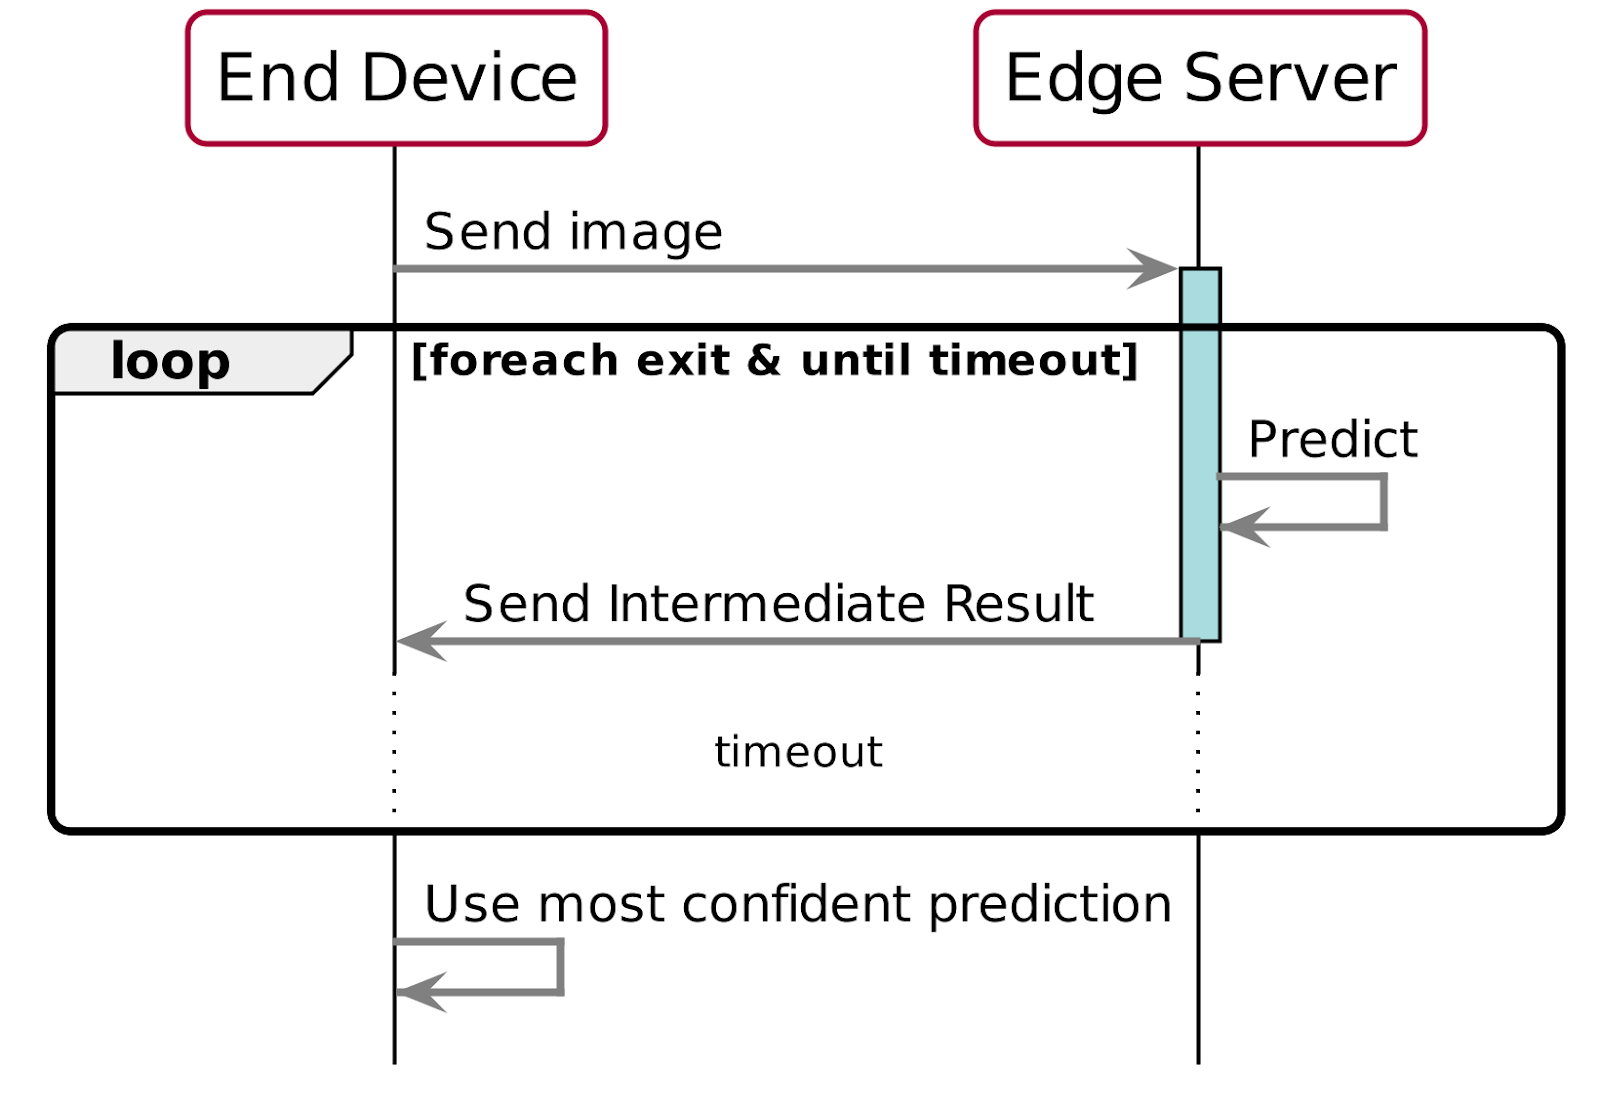
\includegraphics[width=.7\linewidth]{figures/models/sequence_diagram}
	\caption[Sequence Diagram \acrshort{aee}]{Sequence Diagram \acrshort{aee}: The client and server establishes a TCP socket connection. The client loads a samples from the \gls{min100} validation set, and streams the sample to the server. The server preprocess the sample and runs the model inference. As soon as, prediction are obtained, a thread is spawned, to stream the results back to the end device. }
	\label{fig:sequence-diagram}
\end{figure}

The implementation is written in \gls{python} using the \gls{python} Socket API \cite{noauthor_socket_nodate}, \gls{pytorch} \cite{paszke_automatic_2017} and \gls{torchvision} \cite{marcel_torchvision_2010}. The client is deployed on the \gls{nuc} and server on \gls{jetson} and \gls{gpu-ws}. The servers are LAN connected to the router and the client is connected over the WLAN.

\paragraph{Information Combination}

We send back the top-5 predictions to allow info-combination and reduce the data size of the reply. We use top-5, since the correct class is within these 5 predictions close to 90 \% of the time having just two predictions available for any of the models, see figure \ref{fig:top-5-cumulative}.

To combine top-5 prediction information from $ n $ exits, we must expand the vectors back to the original class space of $ C $ dimensions.

Each exit outputs two 5-dimensional vectors. $\mathbf{c}_{i,k}^{top5}$ contains the labels of the top-5 predictions and $ \mathbf{\hat{y}}_{i,k}^{top5}$ contain the class scores of the top-5 predictions. 

\begin{align}
\begin{split}
\mathbf{c}_{i,n}^{top5} &= \begin{bmatrix}
c_{i,n}^{1st} & \phantom{.}c_{i,n}^{2nd} & \phantom{.}c_{i,n}^{3rd} & \phantom{.}c_{i,n}^{4th} & \phantom{.}c_{i,n}^{5th}
\end{bmatrix}, \\
\mathbf{\hat{y}}^{top5}_{i,n} &= \begin{bmatrix}
\hat{y}_{i,n}^{1st} & \hat{y}_{i,n}^{2nd} & \hat{y}_{i,n}^{3rd} & \hat{y}_{i,n}^{4th} & \hat{y}_{i,n}^{5th}
\end{bmatrix}
\end{split}
\end{align}

The vectors are sorted from highest to lowest, hence the score $ \hat{y}_{i,k}^{1st} $ is associated the class label $ c_{i,k}^{1st} $ etc. 

We define an expansion function, which takes the top-5 score vector $ \mathbf{\hat{y}}_{i,n}^{top5}$ and top-5 class label vector  $\mathbf{c}_{i,n}^{top5}$ as input  $ f_{expand}\left(\bm{\hat{y}}_{i,n}^{top5},\mathbf{c}_{i,n}^{top5}\right) $ and outputs a $ C $-dimensional score vector, with the scores value at corresponding class index of the label vector, with the remaining indices are zero.
\begin{align}
f_{expand}\left(\bm{\hat{y}}_{i,n}^{top5},\mathbf{c}_{i,n}^{top5}\right) = 
\begin{bmatrix}
\hat{y}_{i,n,1} & \hat{y}_{i,n,2} & \hat{y}_{i,n,c} & \dots & \hat{y}_{i,n,C}
\end{bmatrix}_{1 \times C}
\end{align}


\subparagraph{Example: Expansion of a 10 class problem} 
\blockquote[]{	 	
	For this classification example, the number of classes $C=10$. From a prediction we get the two output vectors $\mathbf{l}_{i,n}^{top5}$ and $ \mathbf{\hat{y}}_{i,n}^{top5}$.
	\begin{align*}
	\mathbf{c}_{i,n}^{top5} &= \begin{bmatrix}
	\phantom{0}0\phantom{.0} & \phantom{0}3\phantom{.0} & \phantom{0}6\phantom{.0} & \phantom{0}8\phantom{.0} & \phantom{0}9\phantom{.0}
	\end{bmatrix},\\
	\mathbf{\hat{y}}_{i,n}^{top5} &= \begin{bmatrix}
	0.80 & 0.10 & 0.05 & 0.03 & 0.01
	\end{bmatrix}
	\end{align*}
	We use our expansion function $ f_{expand}\left(\bm{\hat{y}}_{i,n}^{top5},\mathbf{c}_{i,n}^{top5}\right) $, which return the score vector $ \mathbf{\hat{y}}_{i,n}$.
	\begin{align*}
	\mathbf{c}_{i,n} &= \begin{bmatrix}
	\phantom{0}0\phantom{.0} & \phantom{0}1\phantom{.0} & \phantom{0}2\phantom{.0} & \phantom{0}3\phantom{.0} & \phantom{0}4\phantom{.0} & \phantom{0}5\phantom{.0} & \phantom{0}6\phantom{.0} & \phantom{0}7\phantom{.0} & \phantom{0}8\phantom{.0} & \phantom{0}9\phantom{.0}
	\end{bmatrix}_{1 \times 10},\\
	\mathbf{\hat{y}}_{i,n}  &= \begin{bmatrix}
	0.80 & 0.00 & 0.00 & 0.10 & 0.00 & 0.00 & 0.05 & 0.00 & 0.03 & 0.01
	\end{bmatrix}_{1 \times 10}
	\end{align*}
}      

Having multiple score vectors $ \bm{\hat{y}}_{i,1}, \dots, \bm{\hat{y}}_{i,n} $ in the original class space, allow us to formulate a $ n \times C $ score matrix $ \bm{\hat{Y}}_{i}^{n \times C} $.
\begin{align}
	\bm{\hat{Y}}_{i}^{n \times C} =
	\begin{bmatrix}
		\hat{y}_{i,1,1} & \hat{y}_{i,1,2} & \dots & \hat{y}_{i,1,C} \\
		\hat{y}_{i,2,1} & \hat{y}_{i,,2} & \dots & \hat{y}_{i,2,C} \\
		\vdots & \vdots & \ddots & \vdots \\
		\hat{y}_{i,n,1} & \hat{y}_{i,n,2} & \dots & \hat{y}_{i,n,C}
	\end{bmatrix}
\end{align}

Formulating as matrix ease the implementation of combination functions to use methods from linear algebra, e.g. finding the maximum entry and summing the columns.

\subparagraph{Example: Prediction matrix and information combination} 
\blockquote[]{	 	
	For this classification example, the number of classes $C=10$. Within a time frame we receive predictions from 3 exits. We assume the predictions have been expanded.
	\begin{align*}
	\mathbf{c}_{i} &= \begin{bmatrix}
	\phantom{0}0\phantom{.0} & \phantom{0}1\phantom{.0} & \phantom{0}2\phantom{.0} & \phantom{0}3\phantom{.0} & \phantom{0}4\phantom{.0} & \phantom{0}5\phantom{.0} & \phantom{0}6\phantom{.0} & \phantom{0}7\phantom{.0} & \phantom{0}8\phantom{.0} & \phantom{0}9\phantom{.0}
	\end{bmatrix}_{1 \times 10},\\
	\mathbf{\hat{y}}_{i,1}  &= \begin{bmatrix}
		0.80 & 0.00 & 0.00 & 0.10 & 0.00 & 0.00 & 0.05 & 0.00 & 0.03 & 0.01
	\end{bmatrix}_{1 \times 10}
	\\
	\mathbf{\hat{y}}_{i,2}  &= \begin{bmatrix}
		0.10 & 0.00 & 0.00 & 0.01 & 0.00 & 0.85 & 0.00 & 0.02 & 0.00 & 0.02
	\end{bmatrix}_{1 \times 10}
		\\
	\mathbf{\hat{y}}_{i,3}  &= \begin{bmatrix}
		0.15 & 0.00 & 0.00 & 0.02 & 0.01 & 0.00 & 0.00 & 0.80 & 0.00 & 0.02
	\end{bmatrix}_{1 \times 10}
	\end{align*}
	We construct the matrix $ \bm{\hat{Y}}_{i}^{n \times C} $
	\begin{align*}
			\bm{\hat{Y}}_{i}^{n \times C} =
		\begin{bmatrix}
		0.80 & 0.00 & 0.00 & 0.10 & 0.00 & 0.00 & 0.05 & 0.00 & 0.03 & 0.01 \\
		0.10 & 0.00 & 0.00 & 0.01 & 0.00 & 0.85 & 0.00 & 0.02 & 0.00 & 0.02 \\
		0.15 & 0.00 & 0.00 & 0.02 & 0.01 & 0.00 & 0.00 & 0.80 & 0.00 & 0.02 
		\end{bmatrix}_{3 \times 10}
	\end{align*}
	We give examples of using the defined combination functions:
	\begin{enumerate}
		\item Using the latest exit prediction the resulting prediction $  \hat{c}^{**}_{i} = \hat{c}^*_{i,3} = 7$.
		\item 	Using the maximum confidence the resulting prediction becomes $ \hat{c}^{**}_{i} =  5$ from exit 2.
		\item 	Using sum confidence we sum all columns to create a new score vector
		\begin{align*}
		\bm{\hat{y}^{**}_{i}} = 
		\begin{bmatrix}
		1.05 & 0.00 & 0.00 & 0.13 & 0.01 & 0.85 & 0.05 & 0.82 & 0.03 & 0.05
		\end{bmatrix}_{1 \times 10}
		\end{align*}
		Thus the resulting prediction becomes $ \hat{c}^{**}_{i} = 0$
		\item Using the score-margin we find the largest difference between the two highest scores in the 2nd row i.e. the second exit. $ f_{margin}\left(\bm{\hat{y}_{i,2}}\right) = \hat{y}_{i,2,5} - \hat{y}_{i,2,0} = 0.85 - 0.10 =0.75 $ Thus the resulting prediction becomes $ \hat{c}^{**}_i = 5$
	\end{enumerate}
	Evidently, combining the scores gives different outcomes in this thought out yet realistic example.
	
}

\section{Results} \label{sec:edge-results}

We want to examine the possibility to combine predictions from multiple exits to obtain a higher accuracy. A study of top-1 predictions results from all exits, revealed that, we too encounter overthinking \cite{kaya_shallow-deep_nodate}, i.e. in some cases an early exit correctly predicts a sample, which a later exit makes wrong. An example is the 6th sample from the \gls{bresnet}, $ c_6 $ is the ground truth class label, $ \hat{c} $ is the predicted class labels, $ \hat{y}^*_6 $ is the corresponding prediction score for the class label at all exits. $ b $ denotes the correctness of each exit as a binary value, where 1 is correct 0 is incorrect.
\begin{align*}
c_6=0,
\mathbf{\hat{c}}_{6}=
\begin{bmatrix}
0 \\
54 \\
62 \\
62
\end{bmatrix},
\mathbf{\hat{y}}^{*}_{6}=
\begin{bmatrix}
0.56 \\
0.32 \\
0.52 \\
0.62
\end{bmatrix} \text{\:and\:}
\mathbf{b}_{6}=
\begin{bmatrix}
1 \\
0 \\
0 \\
0
\end{bmatrix}
\end{align*}
Based on the scores the models is more confident about the last exit prediction, even though the prediction from the first exit is correct. Having all predictions available using the combination functions Latest, max and add will all give the label 62, hence cherry-picking the correct prediction from this set of predictions, is not trivial. Analyzing the exit score have shown, that the score of a later exit is not always higher than the earlier exits, see figure \ref{fig:exit-highscore}.

\begin{figure}
	\captionsetup[subfigure]{justification=centering}
	\centering
	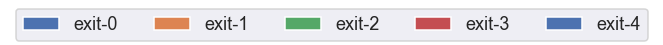
\includegraphics[width=.7\linewidth]{figures/edge/exit0-4_legend}
	\subfloat[B-ResNet]{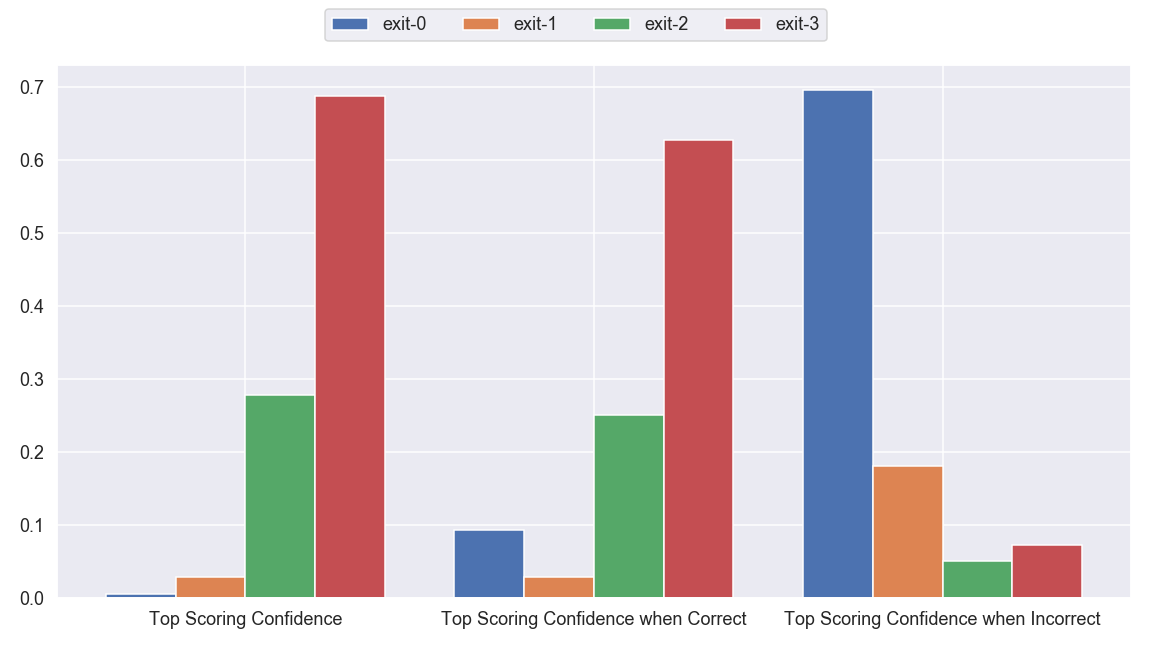
\includegraphics[width=.33\linewidth]{figures/edge/b-resnet_correctness}}
	\hfill
	\subfloat[B-DenseNet]{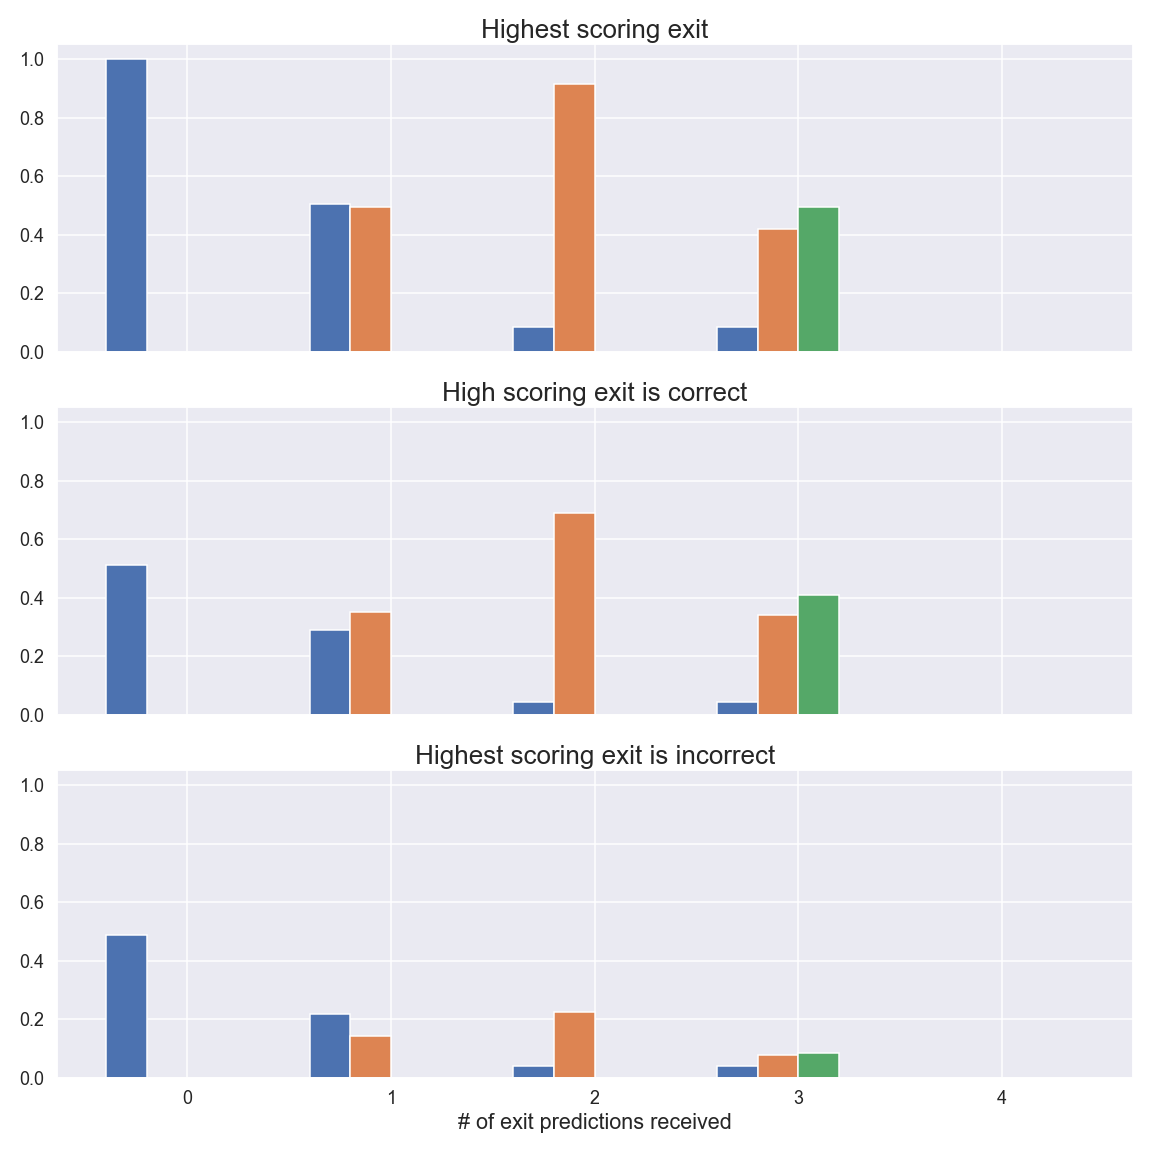
\includegraphics[width=.33\linewidth]{figures/edge/b-densenet_correctness}}
	\hfill
	\subfloat[MSDNet]{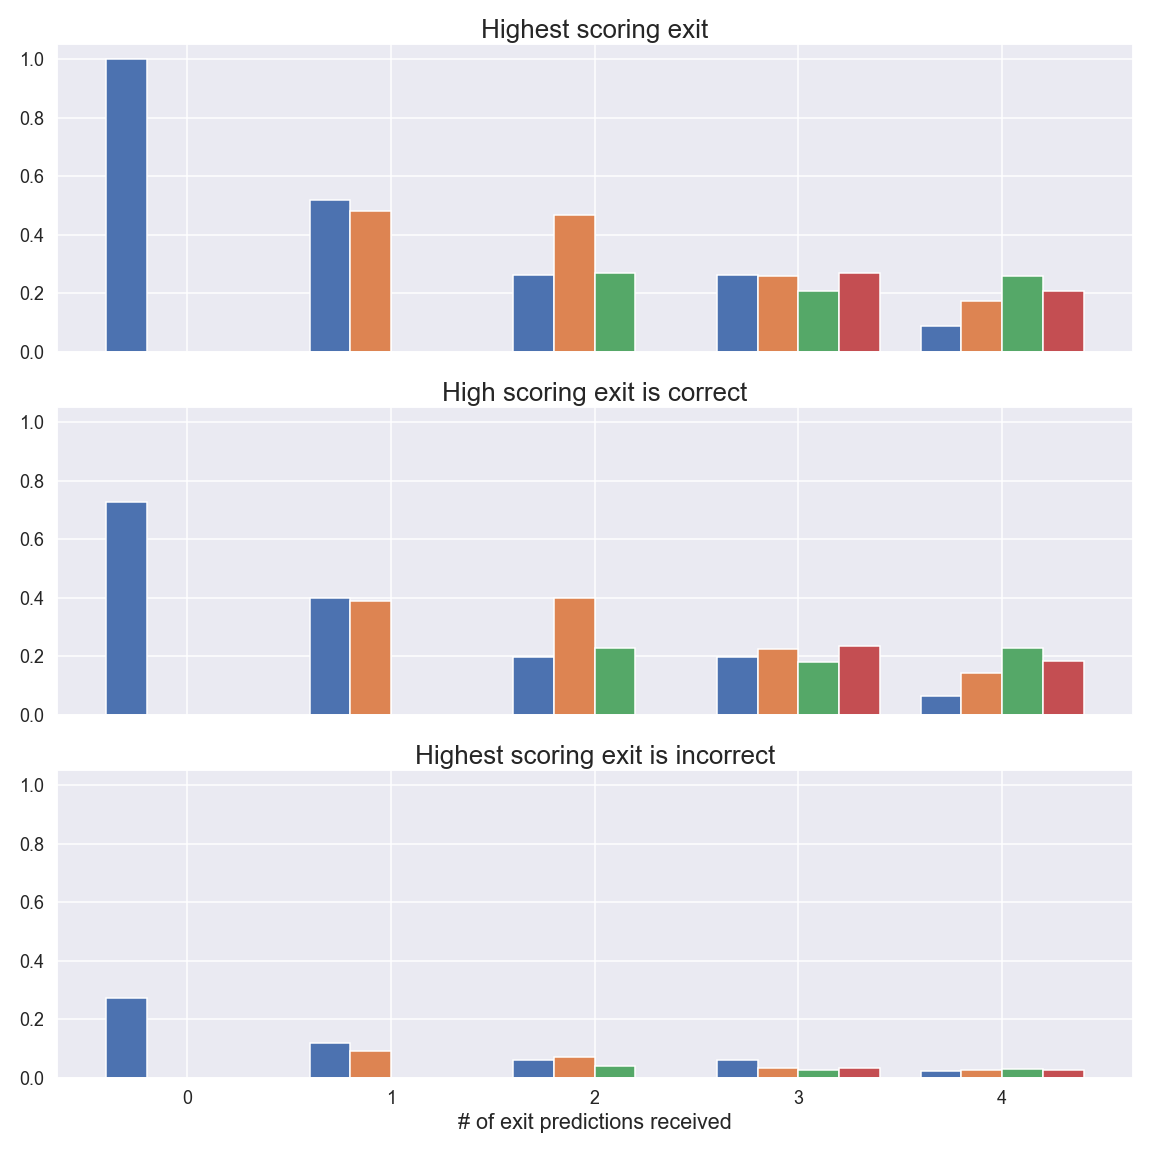
\includegraphics[width=.33\linewidth]{figures/edge/msdnet_correctness}}
	\caption[Model Highest Scoring Exit]{Model Highest Scoring Exit}
	\label{fig:exit-highscore}
\end{figure}

In fact, using the maximum score, as proposed in\cite{kaya_shallow-deep_nodate}, actually reduces the accuracy of the model, see table \ref{tbl:latest-vs-max}. It seems, that although the early exits achieve a higher score, they also introduces more uncertainty.  

\begin{longtabu}{>{\bfseries}X|X|X}
	\caption[]{} \label{tbl:latest-vs-max} \\
	\toprule
	\rowfont{\bfseries}
	Model & latest exit & max score   \tabularnewline
	\bottomrule
	\endfirsthead
	\multicolumn{3}{@{}l}{\textbf{\textcolor{black}{Table \ref{}:}} continued}\\
	\toprule
	\rowfont{\bfseries}
	Model & $Exit_N$ & max score    \tabularnewline
	\bottomrule
	\endhead % all the lines above this will be repeated on every page
	\bottomrule
	\multicolumn{3}{@{}l}{continued \ldots}\\
	\endfoot
	\hline
	\endlastfoot
	B-Resnet	& 0.8826	& 0.8794  \tabularnewline
	\hline
	B-DenseNet	& 0.8660 	& 0.8602 \tabularnewline
	\hline
	MSDNet		& 0.8640 	& 0.8598 \tabularnewline							
	\bottomrule
\end{longtabu}

Figure \ref{fig:exit-highscore} shows the distribution of highest scoring exit given the amount of prediction received, and whether the the highest score is correctly and incorrectly classified. The question is, if using top-5 scores from each exit, we can combine the scores to more confidently selecting the correct prediction among, to obtain a higher accuracy. Figure \ref{fig:top-5-cumulative} plots the top-5 accuracy against a cumulative top-5, that contains the top-5 from all previous exits. 

\begin{figure}
	\centering
	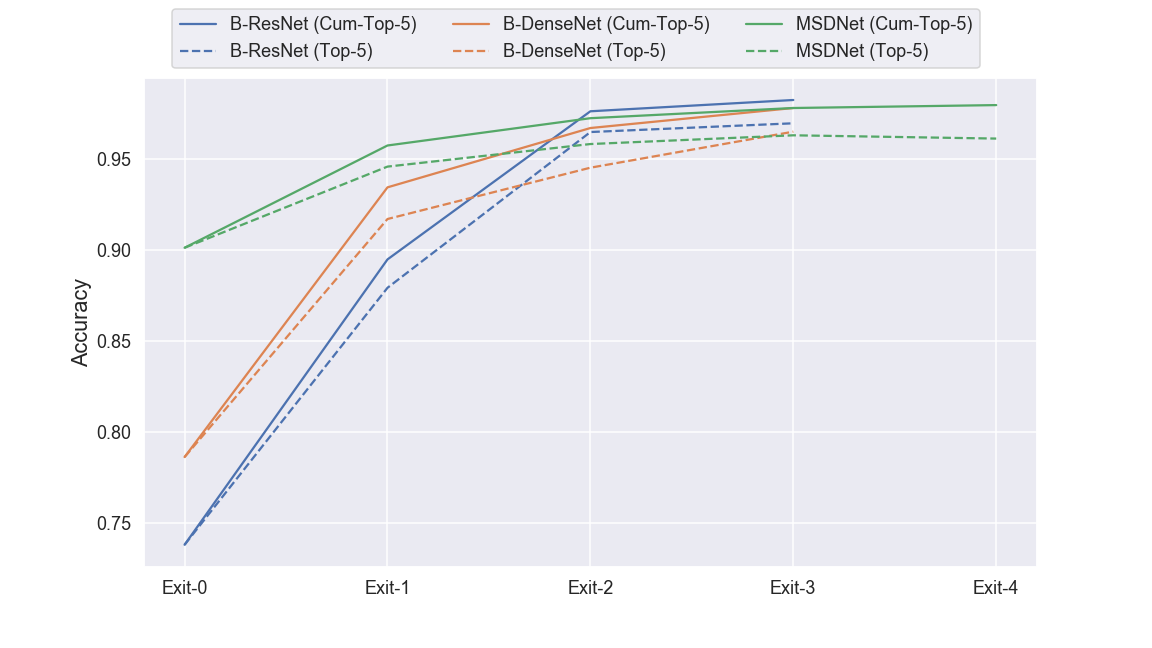
\includegraphics[width=.8\linewidth]{figures/edge/top5cumulative}
	\caption[Top-5 Cumulative]{Model Cumulative Top-5 Accuracy}
	\label{fig:top-5-cumulative}
\end{figure}

From the figure we can tell, that having multiple predictions does indeed improve the cumulative top-5. In the next section we apply the information combination functions to data obtain from running the early exit model and collecting the output scores. 

\subsection{Theoretical Information Combination Analysis}

Using the defined methods to combine the prediction information from multiple exits, as efforts to improve the overall model accuracy, is shown in figure \ref{fig:theoretical-info-combi}. The figure shows the obtainable accuracy given the number of exit predictions received. The blue line \textit{optimum-top5} show the maximum achievable accuracy, if we were always able to pick the right class among the cumulative top-5. The orange line, \textit{optimum-top1}, show the optimal line if, we were always able to pick the correct class among the cumulative top-1 predictions. None of the propose combination methods are able to improve the accuracy, when predictions from all exits is not available. Only the MSDNet shows a small improvement when adding predictions score, when all predictions are available.

\begin{figure}
	\captionsetup[subfigure]{justification=centering,farskip=1pt,captionskip=1pt}
	\centering
	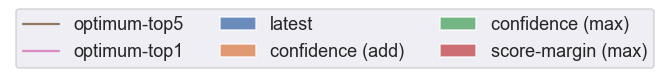
\includegraphics[width=.7\linewidth, keepaspectratio]{figures/edge/theoretical_score_combination_legend}
	\subfloat[B-ResNet]{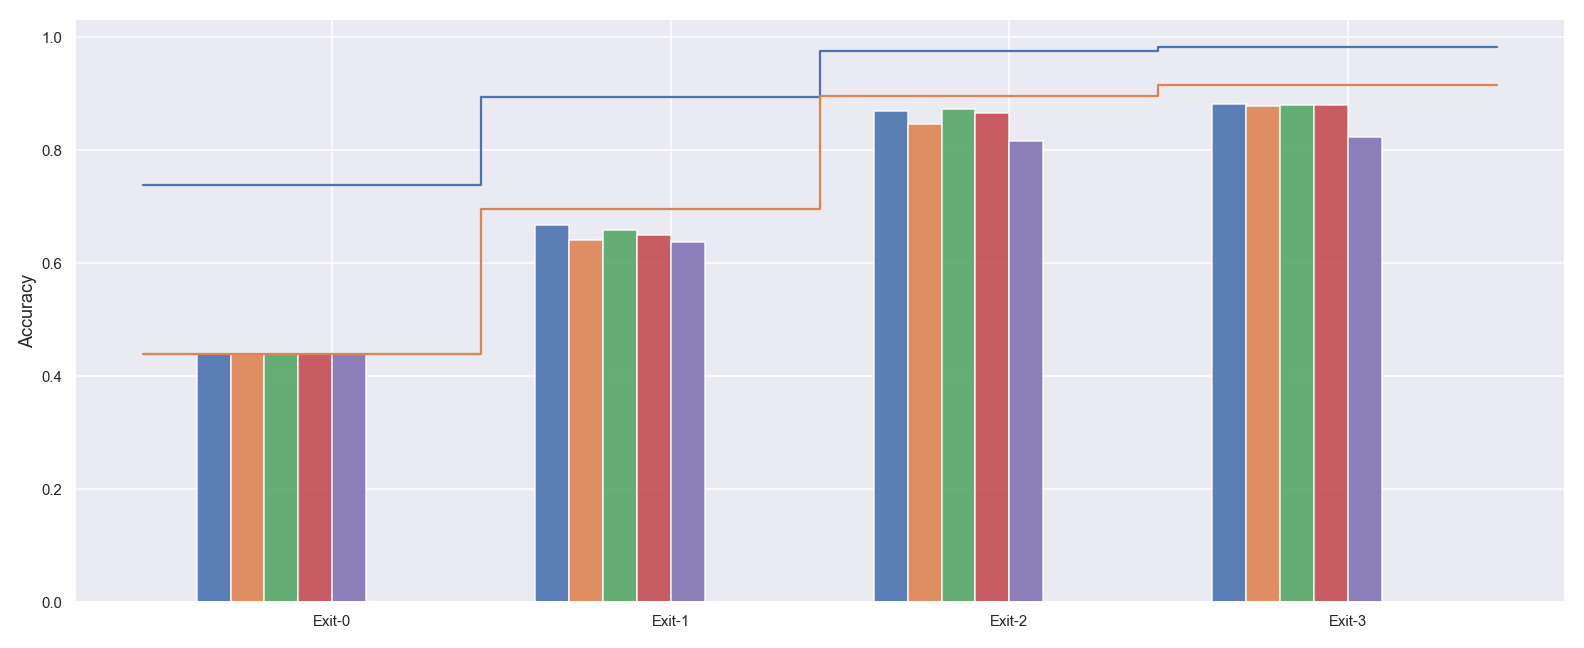
\includegraphics[height=.22\textheight, keepaspectratio]{figures/edge/b-resnet_theoretical_score_combinations}}
	\hfill
	\subfloat[B-DenseNet]{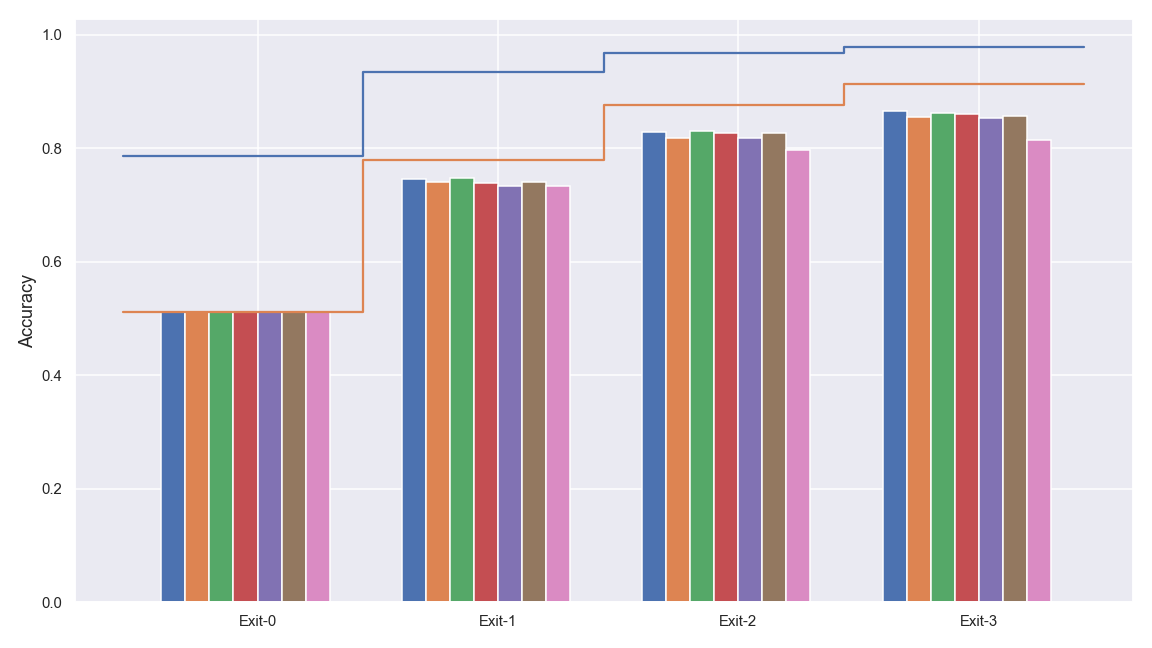
\includegraphics[height=.22\textheight, keepaspectratio]{figures/edge/b-densenet_theoretical_score_combinations}}
	\hfill
	\subfloat[MSDNet]{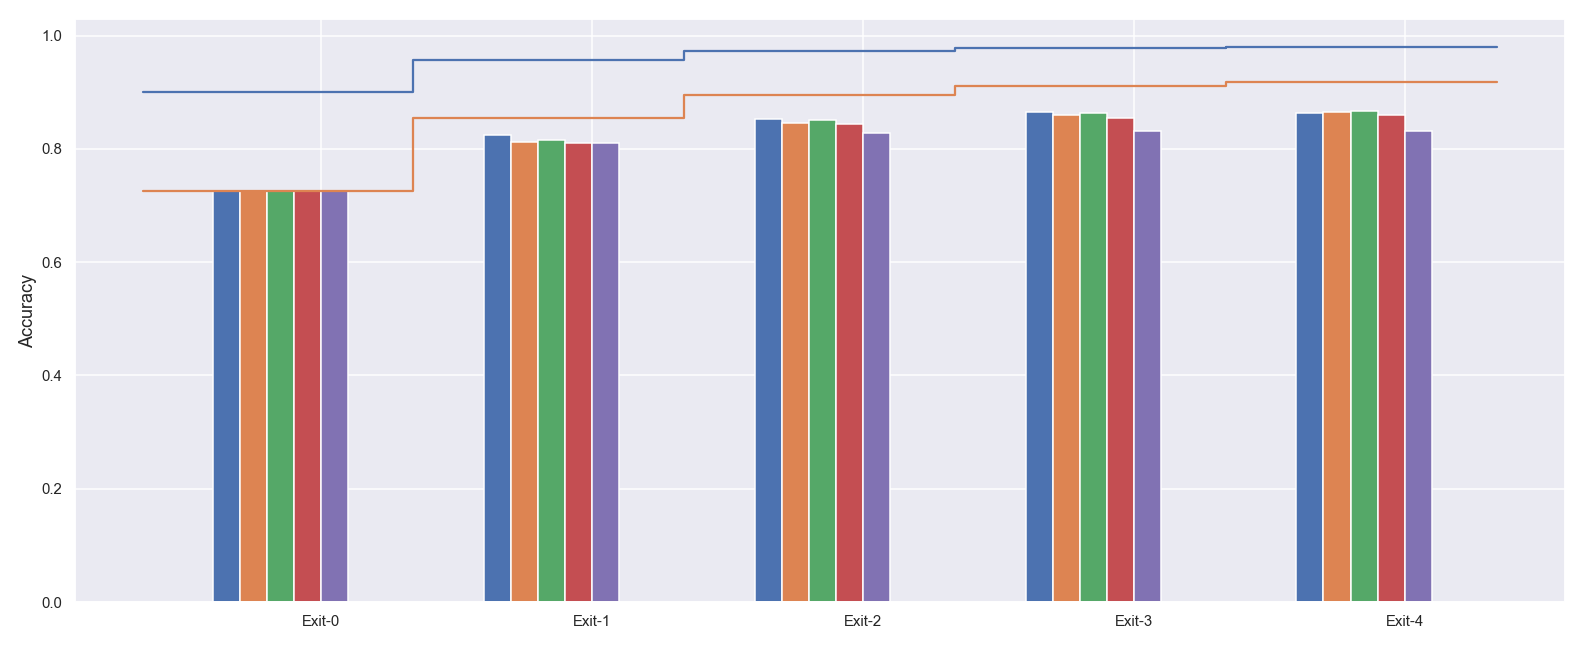
\includegraphics[height=.22\textheight, keepaspectratio]{figures/edge/msdnet_theoretical_score_combinations}}
	\caption[Combination Function with $ n $ Available Exits]{Combination Function with $ n $ Available Exits}
	\label{fig:theoretical-info-combi}
\end{figure}



\subsection{Edge Offloading: \gls{aee} vs Conventional Offloading}

We run test where the images are offloaded from NUC to Jetson. We set different delay threshold and plot the achievable reliability using the prediction from the latest exit, see figure \ref{fig:practical-offloading}. If we compare with figure \ref{fig:delay-threshold}, we obtain less sharp steps, in the areas where a new exit begin to be obtainable, due to the added deviation from the communication. Given this figure, we can select the proper model under different delay threshold, be always selecting the model achieving the highest reliability.  

\begin{figure}
	\captionsetup[subfigure]{justification=centering,farskip=1pt,captionskip=1pt}
	\centering
	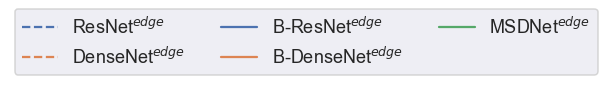
\includegraphics[width=.5\linewidth]{figures/edge/offloading_legend}
	\subfloat[\gls{jetson}]{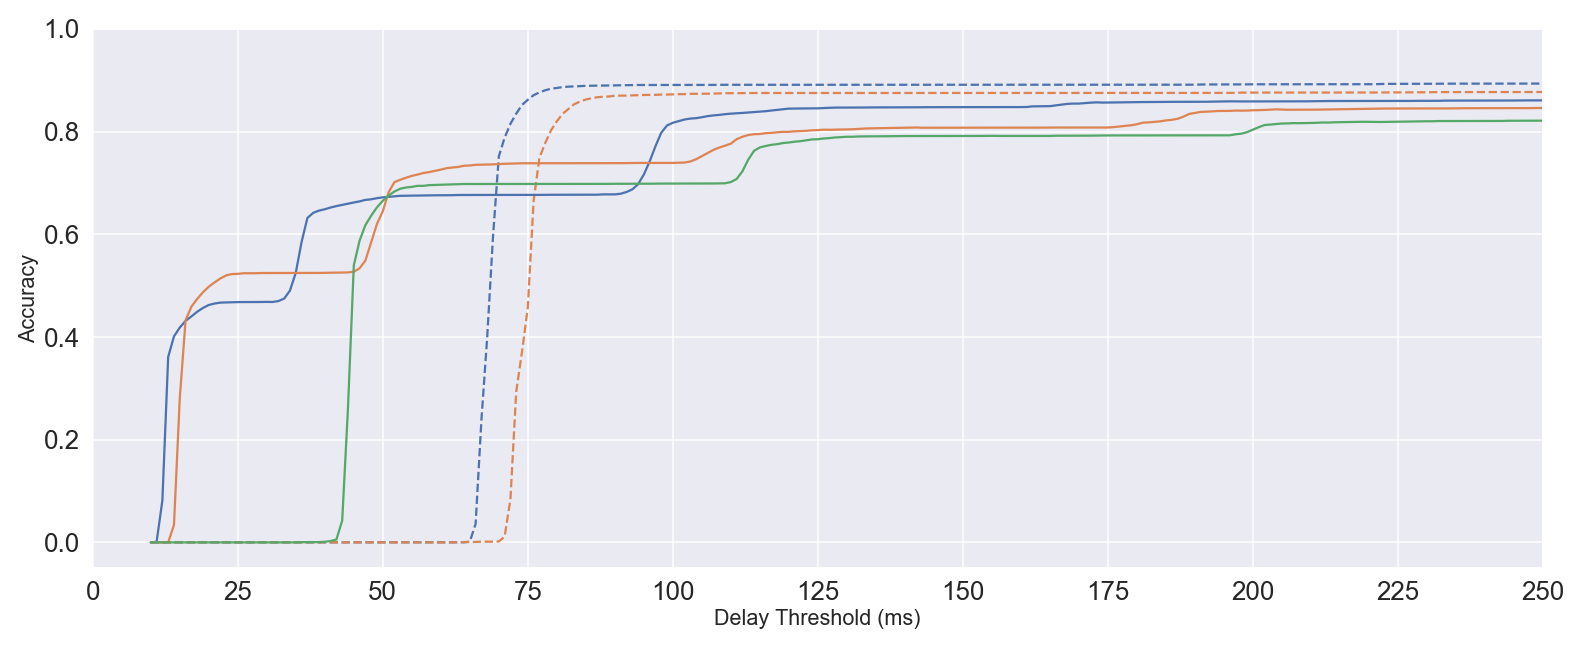
\includegraphics[width=.8\linewidth]{figures/edge/jetson_offloading}}
	\hfill
	\subfloat[\gls{gpu-ws}]{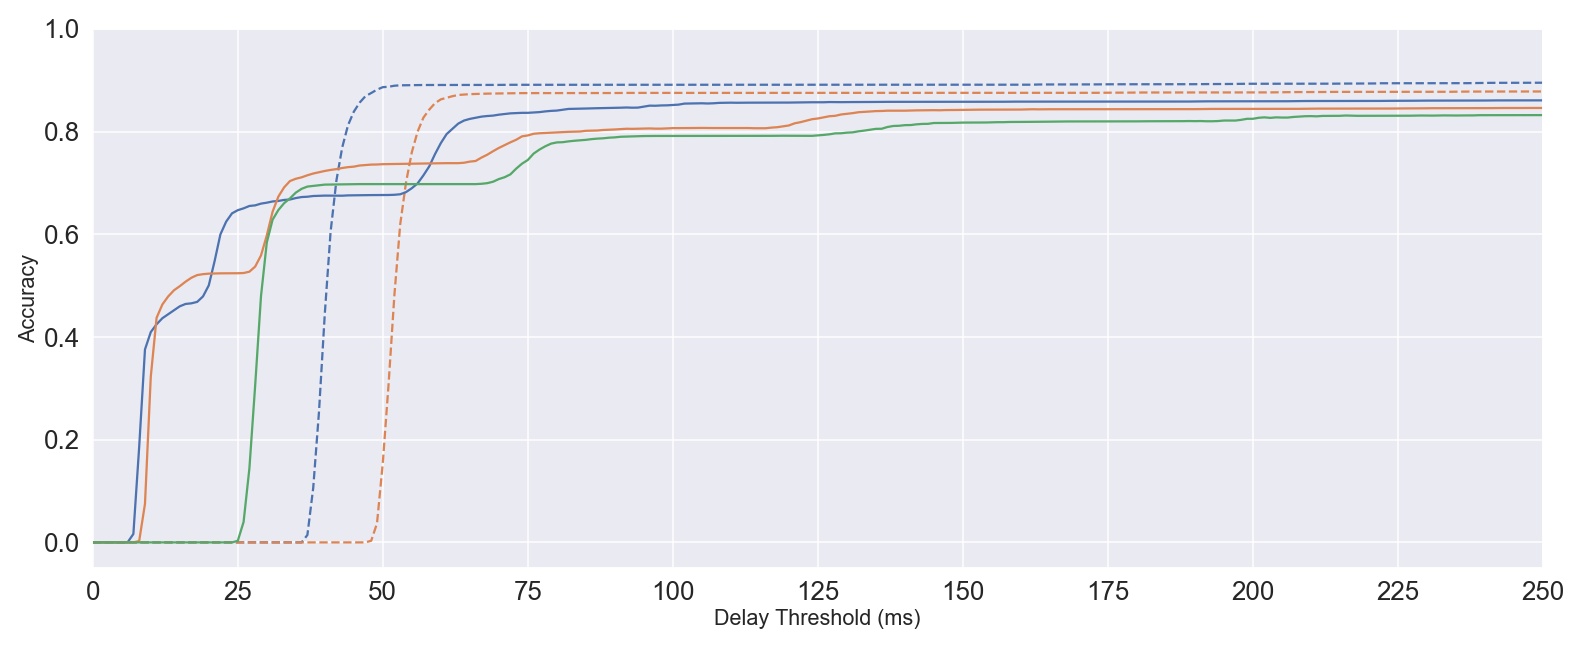
\includegraphics[width=.8\linewidth]{figures/edge/gpu_offloading}}
%	\subfloat[Local Jetson TX2]{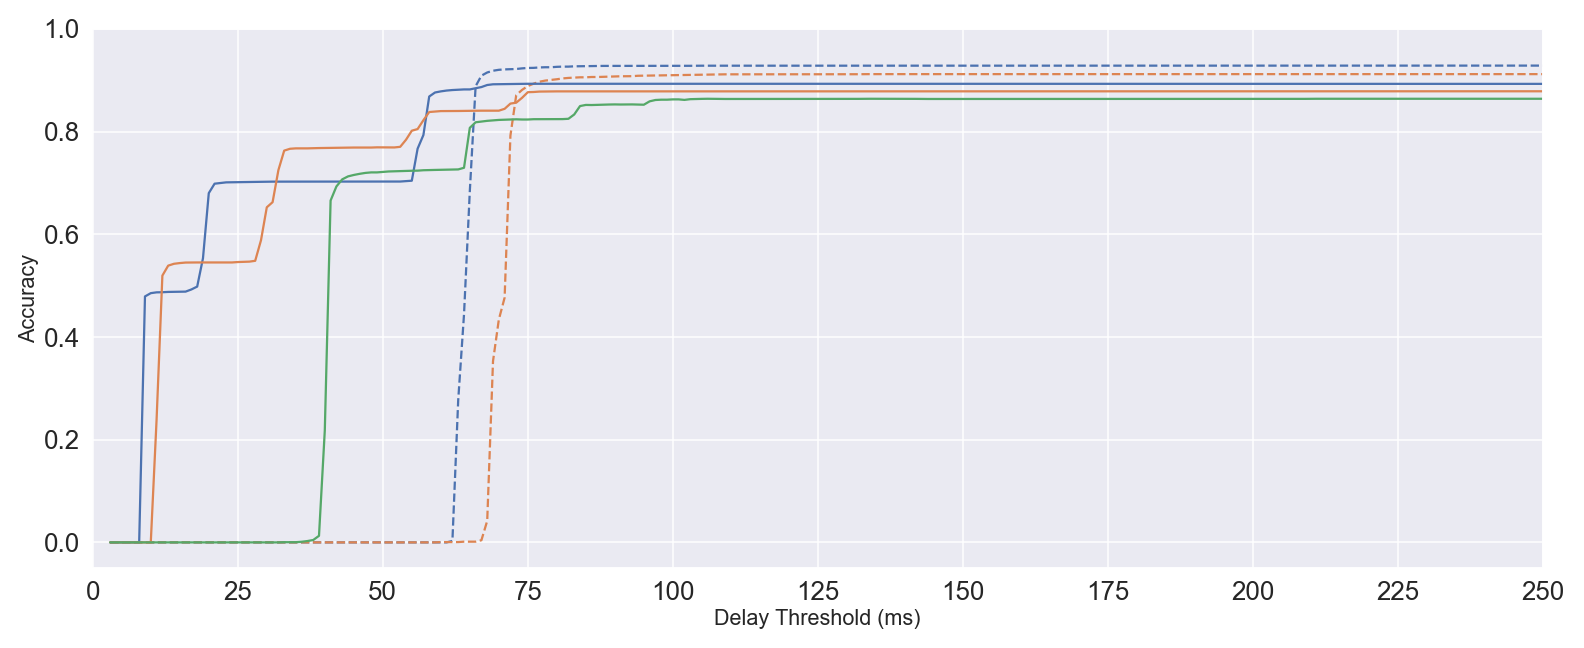
\includegraphics[width=\linewidth]{figures/delay_plots/jetson__delay_threshold}}
	\caption[Offloading NUC to Jetson]{Offloading NUC to Jetson}
	\label{fig:practical-offloading}
\end{figure}

In table \ref{tbl:time-offloading} we present the measured communication time stats, mean, standard deviation, minimum- and maximum value. From the table we see the largest deviation, which support our assertion of the softer steps.  

\begin{longtabu}{>{\bfseries}X|X|X|X|X}
	\caption[]{} \label{tbl:time-offloading} \\
	\toprule
	\rowfont{\bfseries}
	 & \multicolumn4{c}{Communication Time (ms)}    \tabularnewline
	 \tabucline{2-5}
	\rowfont{\bfseries} Offloading & Mean & Std. & Min & Max   \tabularnewline
	\bottomrule
	\endfirsthead
	\multicolumn{3}{@{}l}{\textbf{\textcolor{black}{Table \ref{tbl:time-offloading}:}} continued}\\
	\toprule
	\rowfont{\bfseries}
	Offloading & Up- and downlink Communication Time (ms) &    \tabularnewline
	\bottomrule
	\endhead % all the lines above this will be repeated on every page
	\bottomrule
	\multicolumn{3}{@{}l}{continued \ldots}\\
	\endfoot
	\hline
	\endlastfoot
	NUC to Jetson	& 25.68	& 110.93 & 2.35 & 962.76  \tabularnewline						
	\bottomrule
\end{longtabu}

Additionally, we made a measurement of the delay using the reliable transport protocol, \gls{tcp}. In figure \ref{fig:tcp-overhead}, one can see the impact of using \gls{tcp}. In the three different settings (meetingroom, kitchen, and kitchen) the end-device is moved further apart, which reduced the quality of the communication link. In poor communication environment \gls{tcp} can be expected to have a high overhead introduced by required retransmission, thus have a negative impact on the overall delay.  

\begin{figure}
	\centering
	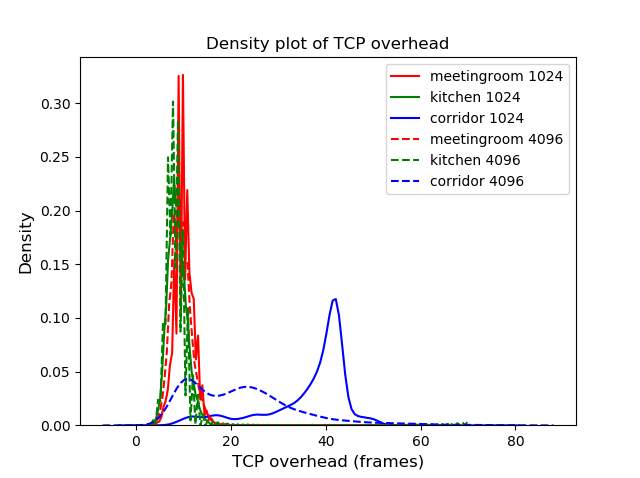
\includegraphics[width=.75\linewidth]{figures/tcp/tcpoverhead}
	\caption[TCP retransmission overhead]{TCP retransmission overhead}
	\label{fig:tcp-overhead}
\end{figure}

We compare running the various model locally on the NUC with offloading to the Jetson, see figure \ref{fig:offloading-vs-local}. Especially under stringent delay thresholds, i.e. the lower region of the plots, we are able to improve the accuracy significantly. However, as the delay threshold are relaxed running locally becomes preferable. One may notice the small drop in reliability, these are cause by extreme delays in the \gls{tcp} protocol, that does not occur locally.

We have conducted experiment with using both \gls{jetson} and \gls{gpu-ws} as edge servers and \gls{nuc} as end device. We compare edge offloading the different models across the two edge platforms and with local inference on the \gls{nuc}. In figure \ref{fig:resnet-offloading-vs-local} we compare the \gls{resnet} based models. In figure \ref{fig:densenet-offloading-vs-local} the \gls{densenet} based models and lastly in figure \ref{fig:msdnet-offloading-vs-local} the \gls{msdnet} model.

\begin{figure}
	\captionsetup[subfigure]{justification=centering, farskip=0pt,captionskip=0pt}
	\centering
	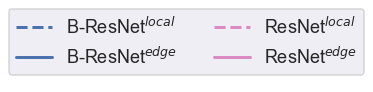
\includegraphics[width=.3\linewidth]{figures/edge/gpu_b-resnet_offloading_vs_local_legend}
	\hfill
	\subfloat[GPU Workstation as Edge\label{fig:resnet-offloading-vs-local-jetson}]{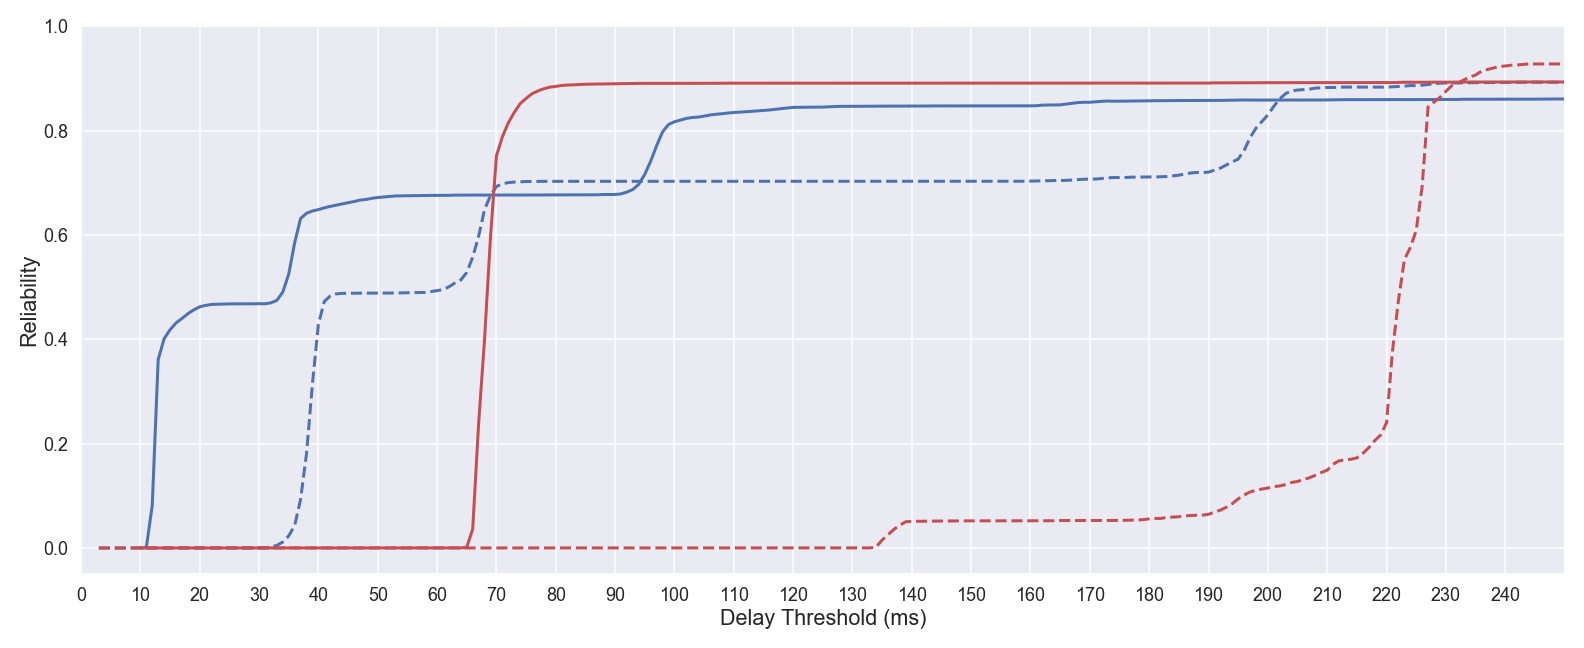
\includegraphics[width=\textwidth,height=.22\textheight,keepaspectratio]{figures/edge/jetson_b-resnet_offloading_vs_local}}
	\hfill
	\subfloat[GPU Workstation as Edge\label{fig:resnet-offloading-vs-local-gpu}]{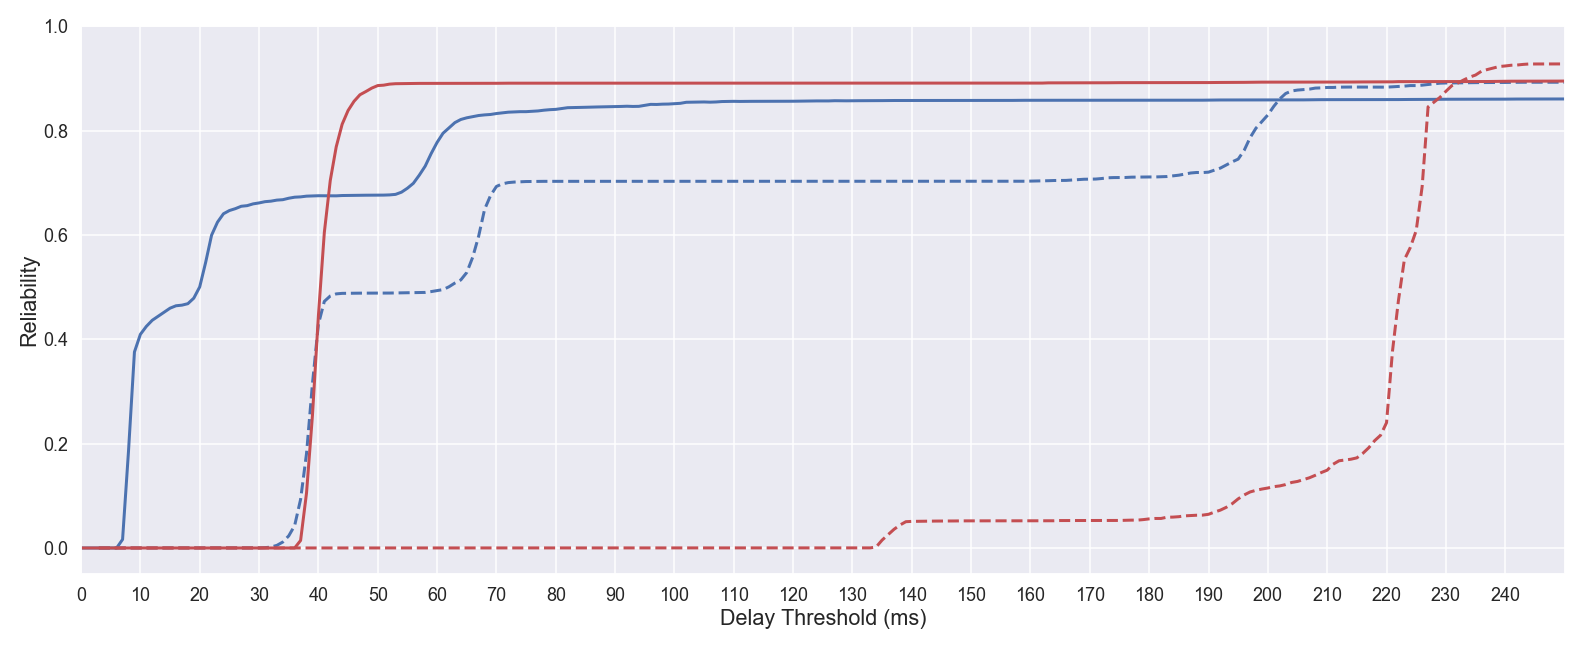
\includegraphics[width=\textwidth,height=.22\textheight,keepaspectratio]{figures/edge/gpu_b-resnet_offloading_vs_local}}
	\caption[Offloading comparison of residual networks]{Offloading comparison of residual networks}
	\label{fig:resnet-offloading-vs-local}
\end{figure}

From figure \ref{fig:resnet-offloading-vs-local} we see, how we are able to improve the reliability under stringent delay requirement using either platform as edge server instead of local inference. We can also see, that we improve the reliability compared to using a conventional model again under stringent requirements. When offloading the conventional model, it starts to outperform the early exit model, if we have above 80ms available using the \gls{jetson} or 50ms available using the \gls{gpu-ws}. Local inference is the best option when having 250 ms available, which is we rarely have. The reason why local execution can obtain a higher reliability, is due to some samples are missed as they do not meet the deadline, this is mostly caused by variations in communication time. 

\begin{figure}
	\captionsetup[subfigure]{justification=centering, farskip=0pt,captionskip=0pt}
	\centering
	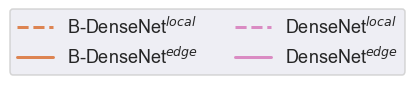
\includegraphics[width=.3\linewidth]{figures/edge/gpu_b-densenet_offloading_vs_local_legend}
	\hfill
	\subfloat[\gls{jetson} as Edge\label{fig:densenet-offloading-vs-local-jetson}]{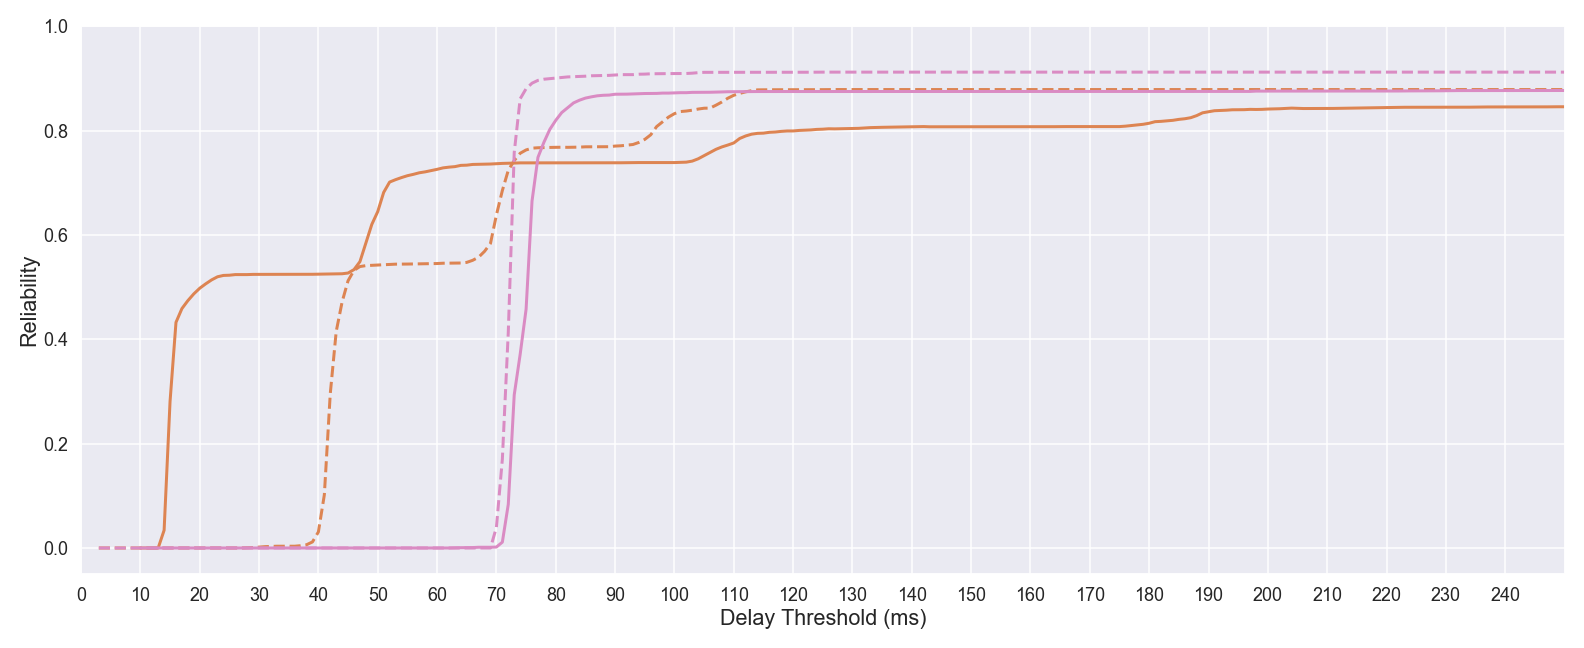
\includegraphics[width=\textwidth,height=.22\textheight,keepaspectratio]{figures/edge/jetson_b-densenet_offloading_vs_local}}
	\hfill
	\subfloat[GPU Workstation as Edge\label{fig:densenet-offloading-vs-local-gpu}]{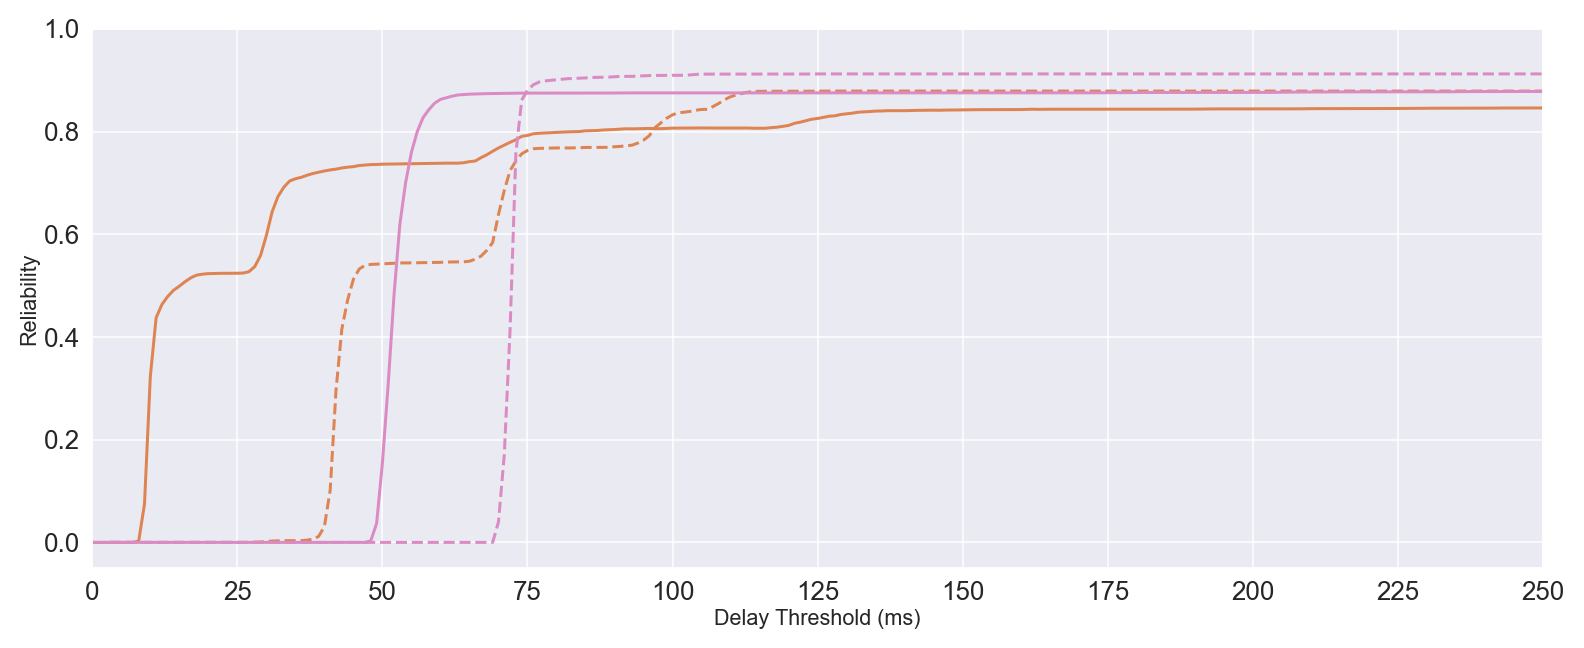
\includegraphics[width=\textwidth,height=.22\textheight,keepaspectratio]{figures/edge/gpu_b-densenet_offloading_vs_local}}
	\caption[Offloading comparison of densely connected networks]{Offloading comparison of densely connected networks}
	\label{fig:densenet-offloading-vs-local}
\end{figure}

The \gls{densenet} tells a somewhat different story. We are still able to improve reliability remarkably under stringent delay requirements using \gls{aee}, compared to offloading a conventional model or locally inference. However, when reaching 70-80 ms on \gls{jetson} all other schemes, local inference B-\gls{densenet} or \gls{densenet} and also offloading \gls{densenet}, starts to outperform \gls{aee}. Local inference of the conventional model is even faster than offloading. The performance difference between the \gls{jetson} and \gls{nuc} is not big enough for the \gls{densenet} based model, this we can tell from looking at \gls{gpu-ws}, where offloading is performing better under 75 ms. 

\begin{figure}
	\captionsetup[subfigure]{justification=centering, farskip=0pt,captionskip=0pt}
	\centering
	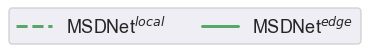
\includegraphics[width=.3\linewidth]{figures/edge/gpu_msdnet_offloading_vs_local_legend}
	\hfill
	\subfloat[GPU Workstation as Edge]{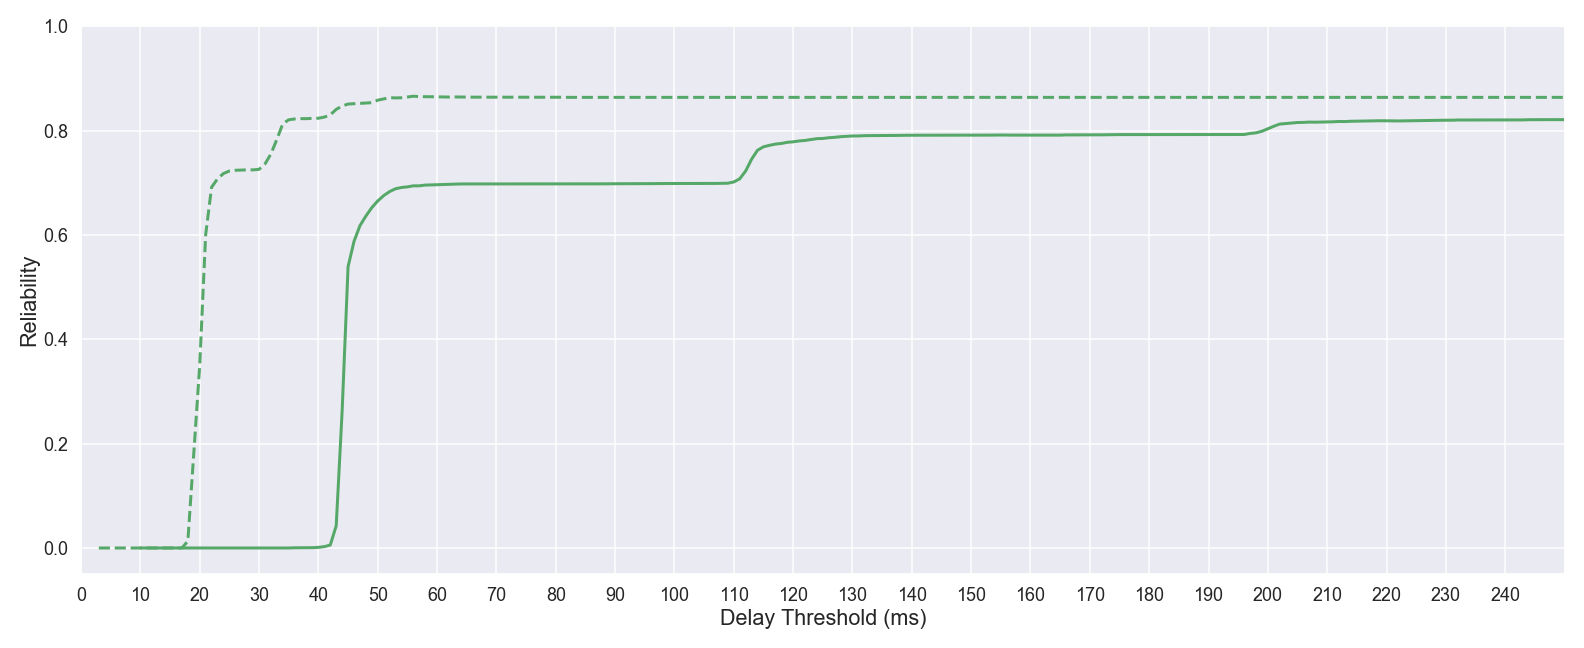
\includegraphics[width=\textwidth,height=.22\textheight,keepaspectratio]{figures/edge/jetson_msdnet_offloading_vs_local}}
	\hfill
	\subfloat[GPU Workstation as Edge]{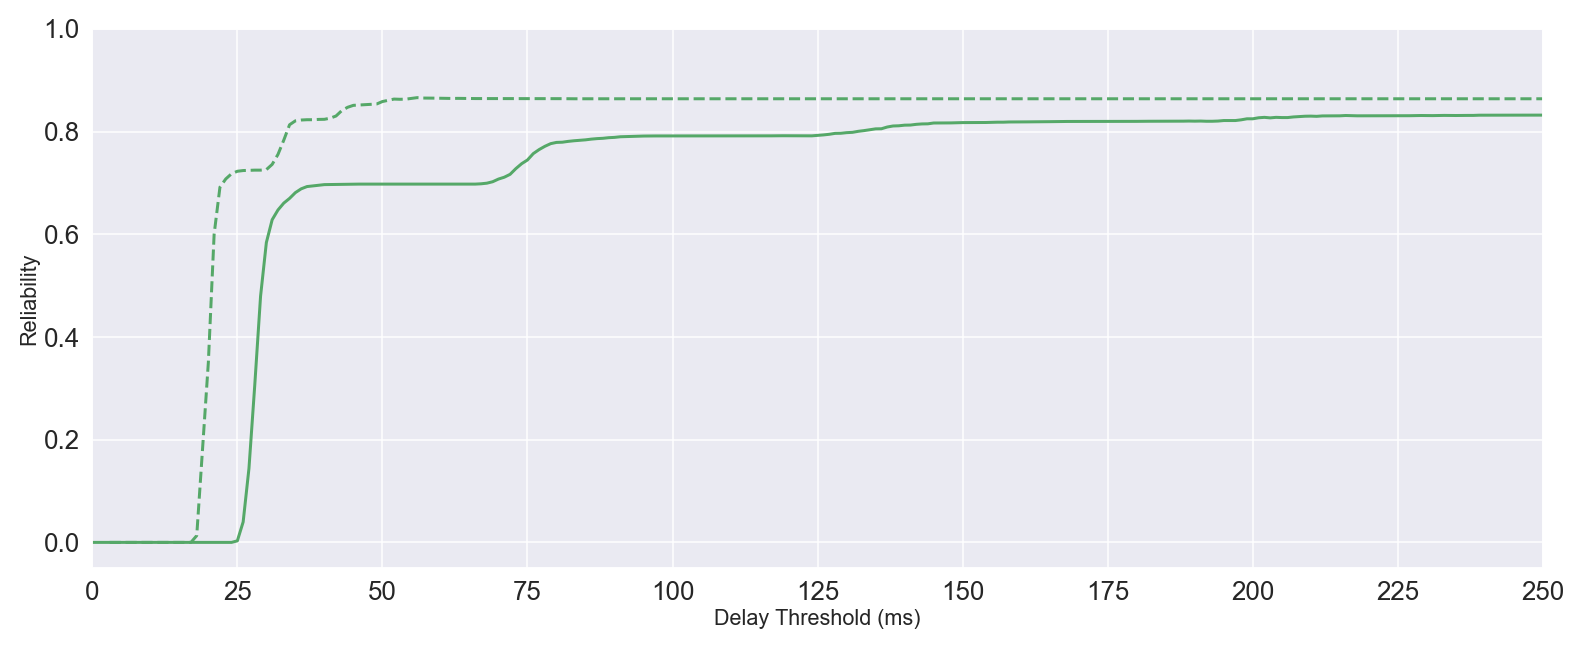
\includegraphics[width=\textwidth,height=.22\textheight,keepaspectratio]{figures/edge/gpu_msdnet_offloading_vs_local}}
	\caption[Offloading comparison of multi-scale dense networks]{Offloading comparison of multi-scale dense networks}
	\label{fig:msdnet-offloading-vs-local}
\end{figure}

\gls{msdnet} tells a completely different story. Local inference is always able to achieve higher reliability irregardless of offloading to \gls{jetson} or \gls{gpu-ws}. We do not elaborate on this tedency, as we saw the same tedency in chapter \ref{ch:earlyexit} and have already discussed it in section \ref{sec:ee-summary}.

\section{Summary} \label{sec:edge-summary}

In this section, we summarize and discuss the results from this chapter. In conclusion of this chapter, we were able to improve the reliability, when using \gls{aee} to run early exit models (B-\gls{resnet} and B-\gls{densenet}) on the edge compared to on-device inference. However, for the \gls{msdnet} our offloading solution was uncompetitive with local execution. The local device i.e. NUC is a very powerful end device equipped with a \gls{cpu}. In reality end device are more likely to be equipped with low-end ARM processors or even smaller processing units. In fact, some end devices may even not be able to run any of the models locally. However, given these results, the edge servers may not necessarily need to be equipped with powerful \gls{gpu}s, as the NUC is able to achieve such high performance running the \gls{msdnet}. Thsee results clearly illustrates the complexity of offloading the inference task of \gls{dnn}, as we were not able to find a single model, that provided the best reliability for all delay threshold. Yet, we did successfully improve the reliability in the sub $ \sim $75 ms range for the \gls{jetson}, and $ \sim $50 ms for the \gls{gpu-ws} using \gls{bresnet} and \gls{densenet}, compared to offloading the inference of a conventional \gls{dnn} and clearly outperformed local inference of both early exit and conventional models. 

Compared to local execution, we see softer breaking point, when time allows to reach a new exit, and we are not able to reach the same accuracy, unless we allow for up to 2 s delays. Communication does indeed introduce a lot of uncertainty, and in some cases it results in lost prediction, that could not satisfy the time-budget. Our evaluation of \gls{tcp} a increasing distance indicates, that using \gls{tcp} leads to a large overhead in retransmission, resulting in additional delay. In chapter \ref{ch:discussion}, we discuss alternatives to reduce the communication latency 

Unfortunately, we did not find a combination function, that was able to improve the accuracy, when only a few predictions were available. In contrast our goal was to improve the accuracy, when all predictions was not available. Only for the \gls{msdnet}, when predictions from all exit were available, were we able to improve the accuracy, but by summing the predictions, using the confidence add function. All exits of this model produces decent prediction accuracy in general, hence less uncertainty from the early exit, whereas the gap between the exit's accuracy of our two other model, \gls{bresnet} and \gls{bdensenet} is larger, thus comes with a lot of uncertainty. We have found, that simply using the latest received predictions, is the best overall choice for these early exit models.

Compared to \gls{ddnn} \cite{teerapittayanon_distributed_2017}, our investigation of \gls{aee} is not used with model partitioning for collaborative edge based. Instead it is based on either local execution or remote offloading, to make full use of computing resource of the more powerful edge server. Still our solution is applicable for collaborative edge, where the end-device locally processes the algorithm up to an early exit and obtains a prediction, then offloads the rest of the execution in a cascaded manner for remote execution. A locally obtained prediction could possibly reduce the amount of missed predictions, if no reply is received from the edge within the time frame. However, we did try partitioning after the first exit, but encountered increased transmission delays and computation time. Further experimenting with this idea was dropped, as it would require implmenting feature compression or \gls{bottlenet} modules to reduce transmission time. Introducing feature compression would additionally require compression-aware retraining, as stated in \cite{choi_near-lossless_2018,choi_near-lossless_2018,eshratifar_bottlenet:_2019}  to avoid experiencing a high cost in accuracy.

It can be justified from looking at figure \ref{fig:resnet-offloading-vs-local} and \ref{fig:densenet-offloading-vs-local}, that show the local inference time of the first exit of \gls{bresnet} and \gls{bdensenet}, is always outperformed by the edge servers. Thus, our choice to not waste idle time on server, by offloading the entire task is the better one for very stringent deadlines. The early layers of the \gls{dnn} is typically also the most demanding, which will lead to worsened inference time exits, and communication of features from the earliest exits, is also heavier than both  features obtained at later exits and sending the compressed image upfront, at least, if no feature compression technique is used.

Instead an alternative solutions to handle the lost prediction dilemma, is a parallel execution of a shallower local \gls{dnn} and a deep remote \gls{dnn} i.e. a parallel Big/Little setup. The end device offloads the compressed image to edge server and in parallel process a smaller and less accurate \gls{dnn} locally. The upside is, that the application can always use the locally obtained prediction and choose to discard it, as more accurate prediction arrives from edge or if a good combination function is found, use the information to choose the best prediction. If offloading is not an possible, then the \gls{aee} offloading is the better option.

We have not considered real-time processing a stream of video frames, but only single image classfication. Comparing our inference scheme \gls{aee} with Edgent, where an upfront selection of exit is to handle the accuracy-latency trade-off. Edgent tries to utilize available time for the frame without postponing the next one. The selection of exit is based on regression models of inference time and a current state of bandwidth. The upfront exit selection is prone to loose predictions caused by unexpected communication delays. Our solutions have higher probability of having received a single prediction, when a timeout occurs. For instance, if the first exit is reachable for \gls{aee}, and if the prediction unexpectedly violates the deadline for a later exit, at least one prediction is available. Whereas for Edgent the same later selected exit, that turned out to not be reachable, then no prediction is received in time. In other words, an early prediction is better than no prediction and only in worst-case where the first exit is unreachable neither \gls{aee} nor Edgent will suffice. We argue, that the potential of early exiting is not fully utilizes by this submodel selection, as the latency overhead of our additional exits classifier is negligible. Additionally such upfront selection also takes some time away from offloading and inference.

Our approach does not address video streaming initially, if we encounter time-out in between to exits the computation is wasted, which optimally could have been used to process the next frame, if received. However, our solution fully utilize the available time, if a next frame is not we received. A future extension to our scheme is to let the server known the deadline and measured bandwidth, and have the server implement a decision based on elapsed time, if the server becomes aware, it cannot reach the next exit, it decides to terminate the inference process, and continue with the next received frame.

Edge/cloud offloading can potentially experience service outage. If an access point is no longer accessible, reconnection delays to a new or the same access point e.g. using WiFi can be expected to take at least 1s \cite{pei_why_2017}. Which will inevitably lead to lost predictions, if no local inference is feasible. If local is feasible we should switch to local execution, when experiences service outages, as in \gls{see} \cite{wang_see:_2019}. \gls{see} is a scheduling scheme to handle on device inference of early exit \gls{dnn}s, if experiencing service outages to offloading services.

\subsection*{Reduce communication time}

The communication latency could possibly be reduced, if the WiFi communication did not go through an access point. Instead the connection could be establish ad-hoc using WiFi Direct. Or we could change the \gls{tcp} transport layer to \gls{udp}.

\gls{tcp} was used for reliable transport to send a single jpeg image for processing, as jpeg is a lossless compression technique, then loosing packets could cause reconstructed images on server-side to be incorrectly classified and reduce the reliability. \gls{tcp} is not designed for video streaming applications, as retransmission of unacknowledged packet increase the communication delay. As shown in figure \ref{fig:tcp-overhead}, \gls{tcp} introduces a large overhead of retransmission, when networking conditions are poor. For video streaming \gls{udp} is more widely used. \gls{udp} is an unreliable protocol, which is applicable in scenarios where some packet loss can be tolerated. For future research streaming either jpeg compressed images over \gls{udp}, as in \cite{liu_maximizing_2019} would be interesting to reduce the communication latency. We did not pursue reducing the communication time, as our focus is not to obtain the best possible results on the development platform, but rather to showcase and tell the story offloading \gls{aee}.

\subsection*{Information Combination} 


Unfortunately, we did not find a combination function, despite they in \cite{kaya_shallow-deep_nodate} show marginal improvements using the highest scoring prediction from all exits. however, in contrast our goal was to improve the accuracy, when all predictions was not available. 
In \gls{ddnn} \cite{teerapittayanon_distributed_2017}, they use a \gls{dnn} to fuse the output from early exits to combine the information. In \gls{ddnn} fused features come from a number of upstream devices, with exits at the same level, where as the sensor fusion in our scenario requires intermediate features of different sizes to be fused, which we do not know is possible or able to improve, hence will require som future research. Additionally it will requires the edge or device to runs this \gls{dnn}, which will cause additional delay  for an operation with possibly limited improvements.\todo{maybe unnecessary}





We argue, that \gls{aee} will in any case achieve at least the same accuracy as upfront exit selection in \cite{li_edge_2018}, even though the exit have been chosen with care, the risk of timeout is still present as both computation and communication delays are not constant. If unexpected delays do occur, it may cause timeouts and lead to lost predictions. However, our scheme reduces the risk of losing prediction by timeout, if an earlier, albeit less accurate predictions is available. 


   



